\subsection{Guadagno Open Loop}

In questa ultima parte dell'esperienza abbiamo cercato di misurare il guadagno $A_{ol}$ del nostro amplificatore reale. Come sappiamo, tale guadagno è una funzione della frequenza. Dobbiamo dunque trovare un modo per misurarlo.

\subsubsection{Misura per basse frequenze}

\begin{wrapfigure}[17]{r}{0.55\textwidth}
  \begin{center}
    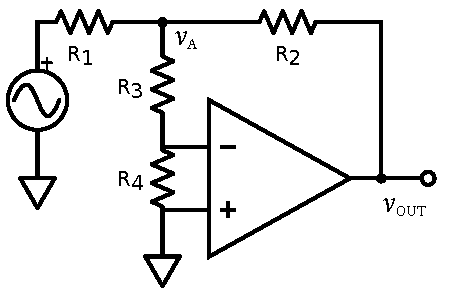
\includegraphics[width=0.280\textwidth]{../E03/latex/LF_ol.pdf}
  \end{center}
  \caption{...}
  \label{cir3:low_frequency}
\end{wrapfigure}


Fino alla frequenza di circa \SI{8}{\hertz} il guadagno di un op-amp $\mu$A741 è di circa $3\times 10^5$. Oltre tale frequenza abbiamo una caduta di circa 20dB/decade. Non risulta dunque possibile effettuare misure a loop aperto in quanto piccolissime variazioni di tensione ai due ingressi causerebbero grandi effetti in uscita. Abbiamo dunque progettato un circuito per ridurre il guadagno in uscita così da non mandare in saturazione il nostro op-amp. In figura (\ref{cir3:low_frequency}) è riportato lo schema circuitale.  

Utilizzando l'oscilloscopio abbiamo misurato i valori di tensione $v_A$ e $v_{out}$. Cerchiamo dunque di legare il guadagno a tali quantità.

Nel caso dell'amplificatore operazionale sappiamo che vale la seguente equazione: $v_{out}=A_{ol}(v_+-v_-)$, dove $v_+$ è la tensione all'ingresso non invertente, $v_-$ la tensione all'ingresso invertente e $A_{ol}$ il guadagno open-loop. Ma $v_+-v_-$ non è altro che la differenza di potenziale presente tra i due ingressi, che sarà ovviamente $\Delta v = I_3R_4$, dove $I_3$ è la corrente che scorre attraverso $R_3$ ed $R_4$\footnote{Assumiamo che la corrente assorbita dagli ingressi sia nulla.}. Possiamo immediatamente stimare tale corrente conoscendo la tensione $v_A$, ovvero $I_3=\frac{v_A}{R_3+R_4}$. 

Trivialmente si ottiene dunque:
\begin{equation}
A_{ol}=\frac{v_{out}}{v_A} \frac{R_4+R_3}{R_4}
\ref{eq3:lfgain}
\end{equation}

Osserviamo come in Eq.\ref{eq3:lfgain} non compaia il termine $V_{in}$. Dovremo dunque scegliere per le varie frequenze una tensione picco-picco in ingresso adeguata in modo che in nostro op-amp non saturi e allo stesso tempo $v_A$ sia sufficientemente grande in modo da essere poco influenzato dal rumore di fondo. 

I valori nominali di resistenza da noi utilizzati sono $R_1=R_2=R_3=\SI{100}{\kilo\ohm}$ e $R_4=\SI{100}{\ohm}$. Per comodità di calcolo abbiamo deciso questa volta di utilizzare il valore nominale con un incertezza del $5\%$. 

Con le resistenze da noi scelte il fattore $\frac{R_4+R_3}{R_4}$ vale circa 1001. Dunque, alla frequenza in cui $A_{ol} \approx 1000 \Rightarrow v_A \approx v_{out}$ 




\subsubsection{Misura per alte frequenze}





